\section{Theseus}

\subsection{Nombre del proyecto o sistema operativo}
El nombre del sistema operativo es ``Theseus''; según \citep{theseus2023intro}, fue nombrado así en honor a la paradoja del barco de Teseo, que plantea la cuestión de, si a un barco le renuevas todas sus piezas, ¿Ese barco renovado sigue siendo el mismo barco? Esta idea de renovación de cada componente es característica de este sistema operativo.

\subsection{Enlace al repositorio y/o documentación oficial}
\begin{itemize}
    \item \textbf{Enlace al repositorio oficial:} https://github.com/theseus-os/Theseus 
    \item \textbf{Enlace al libro oficial:} https://www.theseus-os.com/Theseus/book/index.html
\end{itemize}

\subsection{Objetivo del proyecto}
Según \citep{boos2020theseus}, este sistema operativo es en esencia experimental, aunque puede usarse como objeto de estudio debido a su innovadora arquitectura. También tiene objetivos técnicos, como reestructurar la modularidad, reducir el ``state spill'' y la recuperación ante fallos (fault recovery).

\subsection{Lenguaje(s) de implementación}
Según \citep{boos2020theseus} y confirmando con el repositorio oficial \citep{theseus_GitHub}, el sistema operativo theseus fue casi completamente desarrollado en Rust, aunque también se ha usado C para una futura implementación de la librería ``libc'' dirigida a Theseus (tlibc), ya que por el momento se tomó prestado de la biblioteca de REDOX (relibc).

\subsection{Arquitectura del sistema (monolítica, microkernel, etc.)}
Theseus, como sistema operativo no tiene una arquitectura clásica como monolítica o microkernel, ni mucho menos multikernel; sino que basa su estructura en \textbf{cells} o células por su traducción en español, las cuales haciendo honor a su definición biológica, son módulos pequeños e independientes que sirven como bloque de cons-trucción para el sistema operativo. Adicionalmente, theseus tiene un componente mínimo el cual es llamado ``nano-core'', que se encarga de iniciar el sistema, establecer memoria mínima y cargar las demás células; pero a diferencia de un kernel propiamente dicho, este no es un jefe permanente, sino que cada cell es independiente \citep{boos2020theseus}. A continuación una tabla comparativa entre un kernel clásico y el nano-core de theseus:
\begin{table}[H]
\centering
\caption{Comparación entre un kernel tradicional y el nanocore de Theseus}
\label{tab:nanocore_vs_kernel}
\begin{tabular}{|p{3cm}|p{5.5cm}|p{5.5cm}|}
\hline
\textbf{Aspecto} & \textbf{Kernel tradicional} & \textbf{Nanocore (Theseus)} \\ \hline

\textbf{Definición} &
Es el núcleo del sistema ope-rativo. Centraliza la gestión de componentes y recursos. &
Unidad mínima del núcleo que gestiona sólo lo esencial para iniciar y mantener cells. \\ \hline

\textbf{Estructura} &
Monolítica o microkernel: el kernel controla los servicios del sistema. &
No existe un ``núcleo único'': el sistema está compuesto por módulos cooperativos. \\ \hline

\textbf{Acoplamiento} &
Alto. Los módulos dependen del kernel y de otros subsistemas. &
Bajo. Cada módulo es reemplazable y se comunica mediante interfaces explícitas. \\ \hline

\textbf{Objetivo} &
Proveer servicios centrales de manera estable. &
Eliminar el \textit{state spill} (derrame de estado), permite reemplazar componentes en ejecución. \\ \hline

\end{tabular}

\centering
\small Fuente: Adaptado en base a \citep{boos2020theseus}, \textit{Theseus: An Experiment in OS Structure for State Management}.
\end{table}

Para entenderlo mejor, se especifica que se impone una arquitectura/organización plana para estas células, todo se corre en un solo SAS (single address space) y un solo nivel de privilegio (no se diferencia entre modo usuario y modo kernel) \citep{boos2017theseus}. Además, se incluye una figura comparativa entre arquitecturas clásicas y la de theseus basada en células:
\begin{figure}[H]
\centering
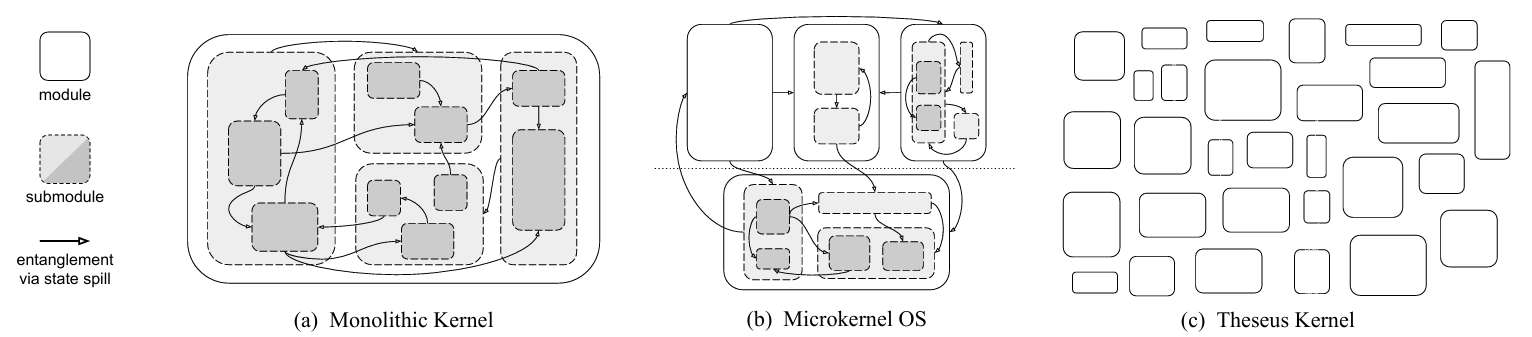
\includegraphics[width=1\textwidth]{figures/comparativaArquitecturaTheseus}
\centering
\caption{Comparativa de la arquitectura de Theseus frente a arquitecturas tradicionales.}
\label{fig:comparativaArquitecturaTheseus}

\centering
\small Fuente: Obtenido de \citep{boos2017theseus} \textit{Theseus: State Spill and OS Structure}.
\end{figure}


\subsection{Componentes implementados (procesos, memoria, archivos, etc.)}

\subsection{Herramientas utilizadas (compiladores, emuladores, etc.)}

\subsection{Nivel de complejidad y accesibilidad para estudiantes}
Considerando un entorno académico, que es justamente donde rust brilla, es un proyecto digno de estudio,
con un alto nivel de complejidad debido sobre todo a su arquitectura mumltikernel; también cabe mencionar que
la dificultad sube debido al uso de (sus herramientas, mencionar)
Sin embargo, se ve compensado debido a su alta accesibilidad, la cual es posible gracias a su extensa documentación 
y estudios en torno a este proyecto.  